\section{Deriving error bounds}
\label{fc-sec:error-bounds}

We now show how to translate the $r$-relaxation to a bound on the error of typical sketches.
We consider two types of error anlayzes of existing sketches. In Section~\ref{fc-ssec:theta-analysis}, we consider the 
relative standard error of the $\Theta$ sketch, which was used in the original analysis of the sketch.  
In Section~\ref{fc-ssec:quantiles-error-analysis} we consider PAC sketches, and show generic error bounds for all $r$-relaxed 
implementations of PAC sketches estimating the number of unique elements and quantiles.  

%We bound the error induced by the relaxation on two representative sketches.
%Section~\ref{fc-ssec:RSE-RMSE} formally defines the RSE and RSME metrics.
%Section~\ref{fc-ssec:theta-analysis} discusses the error introduced to the
%expected estimation and RSE of the KMV $\Theta$ sketch.
%Section~\ref{fc-ssec:quantiles-error-analysis} analyses the PAC Quantiles sketch.



\subsection{\texorpdfstring{$\Theta$}{Theta} error bounds}
\label{fc-ssec:theta-analysis}

We bound the error introduced by an $r$-relaxation of the $\Theta$ sketch over a stream with $n$ unique elements and a parameter (sketch size) of $k$. Given
Theorem~\ref{fc-lemma:opt-genereic-strong}, the optimized concurrent sketch's error is bounded
by the relaxation's error bound for $r=2Nb$. We consider strong and weak adversaries,
${\mathcal{A}}_s$ and ${\mathcal{A}}_w$, resp. For the strong adversary we are able to show only numerical
results, whereas for the weak one we show closed-form bounds. The results are summarized in Table~\ref{fc-table:Theta-Error-Summary}.
Our analysis relies on known results from order statistics~\cite{david2004order}.
It focuses on long streams, and assumes $n>k+r$.

%\begin{table}[H]
%    \begin{tabular}{c|cc|cc|cc}
%                      & \multicolumn{2}{c|}{Sequential sketch} & \multicolumn{2}{c|}{Strong adversary ${\mathcal{A}}_s$} & \multicolumn{2}{c}{Weak adversary ${\mathcal{A}}_w$}   \\[5pt]
%                      & Closed-form& Numerical& \multicolumn{2}{c|}{Numerical} & \multicolumn{2}{c}{Closed-form}   \\[5pt]
%                      \hline
%    Expectation & $n$        & $2^{15}$        & \multicolumn{2}{c|}{$2^{15} \cdot 0.995$}          & \multicolumn{2}{c}{$n\frac{k-1}{k+r-1}$} \\[5pt]
%    RSE & $\leq \frac{1}{\sqrt{k-2}}$        & $\leq 3.1\%$        & \multicolumn{2}{c|}{$\leq 3.8\%$}           & \multicolumn{2}{c}{$\leq 2\frac{1}{\sqrt{k-2}}$}         
%    \end{tabular}
%    \caption{Analysis of $\Theta$ sketch with numerical values for $r=8, k=2^{10}, n=2^{15}$.}
%    \label{fc-table:Theta-Error-Summary}
%\end{table}

\begin{table*}[!ht]
    % Table content (and caption)
    \begin{tabular}{c|cc|cc|cc}
        & \multicolumn{2}{c|}{Sequential sketch} & \multicolumn{2}{c|}{Strong adversary ${\mathcal{A}}_s$} & \multicolumn{2}{c}{Weak adversary ${\mathcal{A}}_w$}   \\%[5pt]
        & Closed-form& Numerical& \multicolumn{2}{c|}{Numerical} & \multicolumn{2}{c}{Closed-form}   \\%[5pt]
        \hline
        Expectation & $n$        & $2^{15}$        & \multicolumn{2}{c|}{$2^{15} \cdot 0.995$}          & \multicolumn{2}{c}{$n\frac{k-1}{k+r-1}$} \\%[5pt]
        RSE & $\leq \frac{1}{\sqrt{k-2}}$        & $\leq 3.1\%$        & \multicolumn{2}{c|}{$\leq 3.8\%$}           & \multicolumn{2}{c}{$\leq 2\frac{1}{\sqrt{k-2}}$}         
    \end{tabular}
    \caption{Expectation and RSE of $\Theta$ sketch with numerical values for $r=8, k=2^{10}, n=2^{15}$.}
    \label{fc-table:Theta-Error-Summary}
\end{table*}

We would like to analyze the distribution of the $k^{th}$ largest element in the 
stream that the relaxed sketch processes, as this determines the result returned by the algorithm. 
We cannot use order statistics to analyze this 
because the adversary alters the stream and so the stream seen by the algorithm is not random.
%the $k^{th}$ largest element in the stream is not a random variable. 
However, the stream of hashed unique elements seen by the adversary \emph{is} random. 
Furthermore, if the adversary hides from the algorithm $j$ elements 
smaller than $\Theta$, then the $k^{th}$ largest element in the stream seen
by the  sketch is the $(k+j)^{th}$ largest element in the original stream seen by the adversary. 
This element is a random variable and therefore we can apply order statistics to it.  

We thus model the hashed unique elements in the stream $A$ processed before a given
query as a set of $n$ labelled iid random variables $A_1,\dots,A_n$, taken uniformly 
from the interval $[0,1]$. Note that
$A$ is the stream observed by the reference sequential sketch, and 
also by adversary that hides up to $r$ elements from the relaxed sketch. 
Let $M_{(i)}$ be the $i^{th}$ minimum value among the $n$ random variables $A_1,\dots,A_n$.

Let $est(x) \triangleq \frac{k-1}{x}$ be the estimate computation
with a given $x=\Theta$ (line~\ref{fc-l:update-est} of Algorithm~\ref{fc-alg:composable-theta}).
The sequential (non-relaxed) sketch returns $e=est(M_{(k)})$.
It has been shown that the sketch is unbiased~\cite{KMV}, i.e., $E[e]=n$ the number of unique elements.
Moreover, previous work~\cite{lee-theta} has analyzed the \emph{relative standard error (RSE)} of the sketch, which is 
the standard error divided by the mean, and has shown it to be  
$\textit{RSE}[e]\leq \frac{1}{\sqrt{k-2}}$.
%the supplementary material Section~\ref{fc-ssec:RSE-RMSE}.
%Because this sketch is unbiased, $\textit{RSE}[e]=$\emph{RSME}$[e]$.

In a relaxed history, the adversary chooses up to $r$ variables to hide from the given query so as to maximize its
error. It can also re-order elements, but the state of a $\Theta$ sketch after a set of updates
is independent of their processing order. Let $M^r_{(i)}$ be the $i^{th}$ minimum value among
the hashes seen by the query, i.e., arising in updates that precede the query in the relaxed history.
The value of $\Theta$ is $M^r_{(k)}$, which is equal to $M_{(k+j)}$ for some $0 \leq j \leq r$.
We do not know if the adversary can actually control $j$,
but we know that it can impact it, %and so to bound the error, we can take the worst possible $j$.
%While an arbitrary set of $r$ updates is hidden, in the $\Theta$ sketch,
%only hidden elements that impact $j$ (have hashes smaller than $M^r_{(k)}$)
%affect the query.
and so for our error analysis, we consider strictly stronger adversaries --
we allow both the weak and the strong adversaries to choose the number of hidden
elements $j$. Our error analysis gives an upper bound on the error induced by our adversaries.
Note that the strong adversary can choose $j$ based on the coin flips,
while the weak adversary cannot, and so it cannot distinguish the algorithm state (set of retained elements) from a random one. Since the state is random in all runs, it chooses the same $j$ in all runs.
%The strong adversary knows the hash function and can select $j$ adaptively; the
%weak adversary does not and therefore chooses the same $j$ in all runs.  
%Note that $j$ counts only hidden elements smaller
%than $\Theta$; others are inconsequential.
We show that the largest error is always obtained either for $j=0$ or for $j=r$.
\begin{claim}
    Consider $j$ values $X_i$, $1 \leq i \leq j$, in the interval $[0,1]$,
    let $M_{(i)}$ be the $i^{th}$ minimum value
    among the $j$. The $X_i$ that maximizes $\abs{\frac{k-1}{x}-n}$ for a given $n$
    is either $M_{(0)}$ or $M_{(j)}$.
    \label{fc-claim:max-val}    
\end{claim}
\begin{proof}
    Assume for the sake of contradiction that the variable that
    maximizes $\abs{\frac{k-1}{x}-n}$ is $M_{(i)}$ for $0<i<j$.  We consider two cases:
    \begin{itemize}
    \item If $\frac{k-1}{M_{(i)}} \leq n$, as $M_{(j)} > M_{(i)}$ then $\frac{k-1}{M_{(j)}} < \frac{k-1}{M_{(i)}} \leq n$,
    therefore $\abs{\frac{k-1}{M_{(j)}}-n} > \abs{\frac{k-1}{M_{(i)}}-n}$, which is a contradiction.
    \item If $\frac{k-1}{M_{(i)}} > n$, as $M_{(0)} < M_{(i)}$ then $\frac{k-1}{M_{(0)}} > \frac{k-1}{M_{(i)}} > n$,
    therefore $\abs{\frac{k-1}{M_{(0)}}-n} > \abs{\frac{k-1}{M_{(i)}}-n}$, which is a contradiction.
    \end{itemize}
\end{proof}


\begin{figure}[b]
%\begin{wrapfigure}{r}{0.4\textwidth}
    \begin{center}
        %\vspace{-0.4in}
        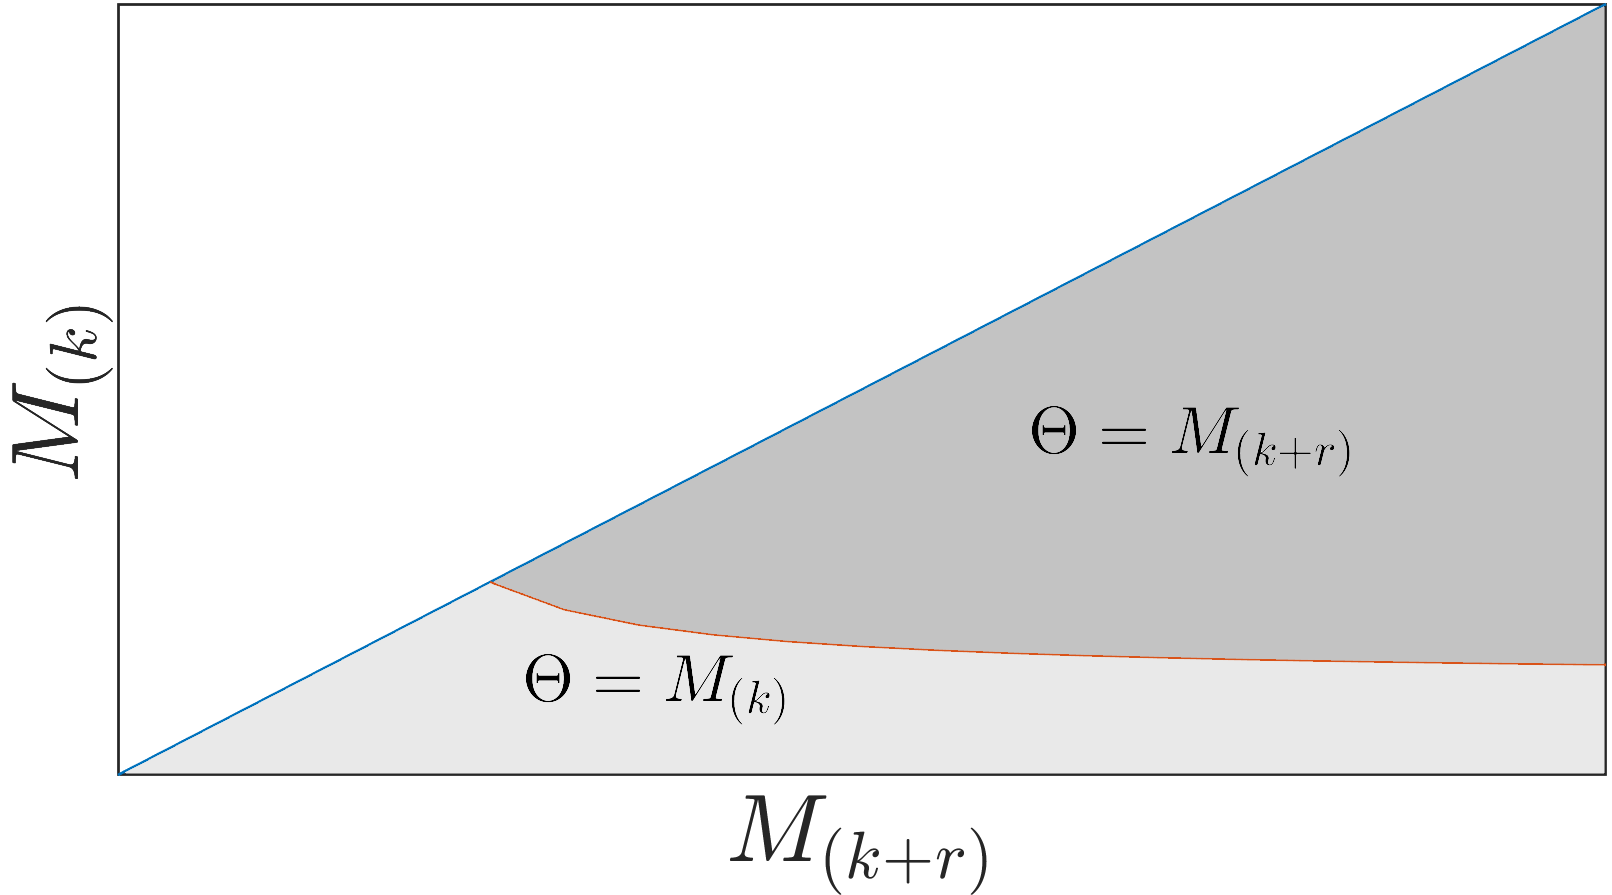
\includegraphics[width=0.38\textwidth]{graphics/fast-concurrent/areaGraph.png}
        %\vspace{-0.2in}
    \end{center}
    \caption{Areas of $M_{(k)}$ and $M_{(k+r)}$. In the dark gray 
    ${\mathcal{A}}_s$ induces $\Theta=M_{(k+r)}$, and in the light gray, $\Theta=M_{(k)}$. The white
    area is not feasible.} %\vspace{-0.1in}
    \label{fc-fig:areaGraph}
%\end{wrapfigure}
\end{figure}

Consider an adversary $\mathcal{A}$ whose estimate is a random variable $e_{\mathcal{A}}$,
characterized by the probability density function $f_{e_{\mathcal{A}}}$.
The expectation of $e_{\mathcal{A}}$ is not necessarily $n$, and so the relative standard error needs to be computed as the error from the desired estimate, $n$, rather than from the expectation. This can be done using the following formula:
\[
    (\textit{RSE}[e_{\mathcal{A}}])^2 = \frac{1}{n^2} \Int_{-\infty}^{\infty} (e - n)^2 \cdot f_{e_{\mathcal{A}}}(e) \,de 
\]
We prove
the following bound:
%Lemma~\ref{fc-lemma:theta-adversary-bound} in the supplementary material Section~\ref{fc-ssec:theta-error-bounds} proves the following bound:
\begin{align*}
    \textit{RSE}[e_{\mathcal{A}}] \leq \sqrt{\frac{\sigma^2(e_{\mathcal{A}})}{n^2}} + \sqrt{\frac{(E[e_{\mathcal{A}}] - n)^2}{n^2}}.
\end{align*}

\begin{lemma}
    The RSE of $e_{\mathcal{A}}$ satisfies the inequality 
    $\textit{RSE}[e_{\mathcal{A}}] \leq \sqrt{\frac{\sigma^2(e_{\mathcal{A}})}{n^2}} + \sqrt{\frac{(E[e_{\mathcal{A}}] - n)^2}{n^2}}$.
    \label{fc-lemma:theta-adversary-bound}
\end{lemma}
\begin{proof}
    \begin{align*}
    \begin{split}
    (\textit{RSE}[e_{\mathcal{A}}])^2 &= \frac{1}{n^2} \Int_{-\infty}^{\infty} (e - n)^2 \cdot f_{e_{\mathcal{A}}}(e) \,de \\
    &= \frac{1}{n^2} \Int_{-\infty}^{\infty} (e - E[e_{\mathcal{A}}] + E[e_{\mathcal{A}}] - n)^2 \cdot f_{e_{\mathcal{A}}}(e) \,de \\
    &\leq \frac{1}{n^2} \Int_{-\infty}^{\infty} \left((e - E[e_{\mathcal{A}}])^2 + (E[e_{\mathcal{A}}] - n)^2 \right)\cdot f_{e_{\mathcal{A}}}(e) \,de \\
    &= \frac{\sigma^2(e_{\mathcal{A}}) + (E[e_{\mathcal{A}}] - n)^2}{n^2} \\
    \text{RSE}[e_{\mathcal{A}}] &\leq \sqrt{\frac{\sigma^2(e_{\mathcal{A}})}{n^2}} + \sqrt{\frac{(E[e_{\mathcal{A}}] - n)^2}{n^2}}
    \end{split}
    \end{align*}
\end{proof}

\paragraph{Strong adversary ${\mathcal{A}}_s$} The strong adversary knows the coin flips in advance, and thus chooses
$j$ to be $g(0, r)$, where $g$ is the
choice that maximizes the error:
\begin{align*}
    g(j_1, j_2) \triangleq \argmax_{j \in \left\{j_1, j_2\right\}} \abs{\frac{k-1}{M_{(k+j)}} - n}.
\end{align*} 

\begin{figure}[b]
%\begin{wrapfigure}{l}{0.4\textwidth}
    \begin{center}
        %\vspace{-0.2in}
        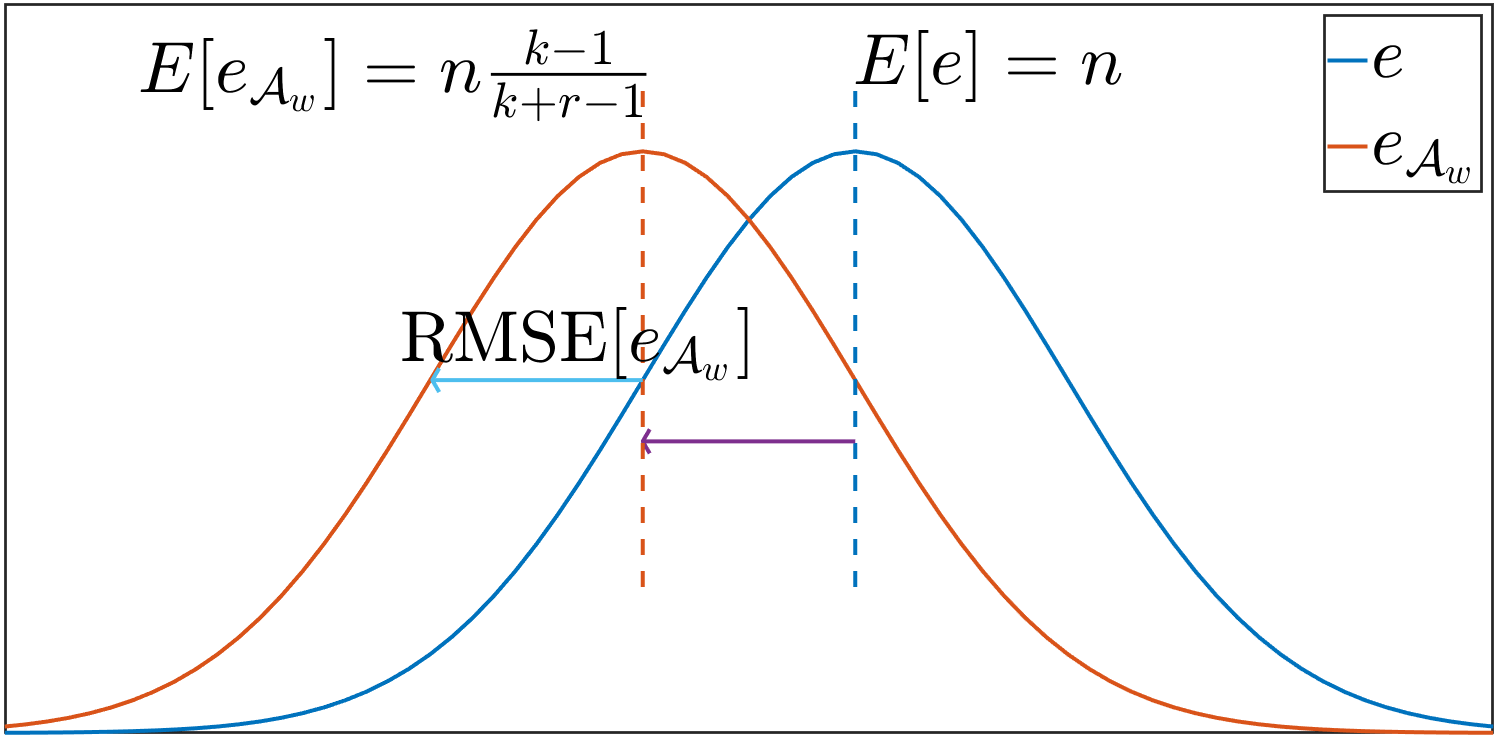
\includegraphics[width=0.39\textwidth]{graphics/fast-concurrent/thetaGraph.png}
        %\vspace{-0.2in}
    \end{center}
    \caption{Distribution of estimators $e$ and $e_{{\mathcal{A}}_w}$. The RSE of $e_{{\mathcal{A}}_w}$ with regards to $n$ is bounded
    by the relative bias plus the RMSE of $e_{{\mathcal{A}}_w}$.}%\vspace{-0.2in}}
    \label{fc-fig:thetaGraph}
%\end{wrapfigure}
\end{figure}

Recall the the ${\mathcal{A}}_s$ knows the oracles coin
flips, therefore knows $M_{(k)}$ and $M_{(k+r)}$, and chooses $M^r_{(k)}$ accordingly. Therefore, our analysis
is on the order statistics of the full stream, as it is this that the adversary sees. From order statistics, the joint probability density
function of $M_{(k)}, M_{(k+r)}$ is:
\begin{align*}
f_{M_{(k)},M_{(k+r)}}(m_k,m_{k+r}) = n!\frac{m_k^{k-1}}{(k-1)!} \frac{(m_{k+r}-m_k)^{r-1}}{(r-1)!}\frac{(1-m_{k+r})^{n-(k+r)}}{(n-(k+r))!}.
\end{align*}

The expectation of $e_{{\mathcal{A}}_s}$ and $e_{{\mathcal{A}}_s}^2$ can be computed as follows:
\begin{equation}
    \begin{split}
    E[e_{{\mathcal{A}}_s}] = \Int_{0}^{1} \Int_{0}^{m_{k+r}} e_{{\mathcal{A}}_s} \cdot f_{M_{(k)},M_{(k+r)}}(m_k,m_{k+r}) \,dm_{k}\,dm_{k+r} \\
    E[e_{{\mathcal{A}}_s}^2] = \Int_{0}^{1} \Int_{0}^{m_{k+r}} \left[e_{{\mathcal{A}}_s} \right] ^2 \cdot f_{M_{(k)},M_{(k+r)}}(m_k,m_{k+r}) \,dm_{k}\,dm_{k+r}
    \end{split}
    \label{fc-eq:strong-expectation}
\end{equation}
Finally, the RSE of $e_{{\mathcal{A}}_s}$ is derived from the standard error of $e_{{\mathcal{A}}_s}$:
\begin{equation}
    \begin{split}
    \text{RSE}[e_{{\mathcal{A}}_s}]^2 &= \frac{1}{n^2}\Int_{0}^{1} \Int_{0}^{m_{k+r}} \left( e_{{\mathcal{A}}_s} - n \right)^2 \cdot f_{M_{(k)},M_{(k+r)}}(m_k,m_{k+r}) \,dm_{k}\,dm_{k+r} \\
    &= \frac{1}{n^2} \Int_{0}^{1} \Int_{0}^{m_{k+r}} \left( e_{{\mathcal{A}}_s} -E[e_{{\mathcal{A}}_s}] + E[e_{{\mathcal{A}}_s}] - n \right)^2 \cdot f_{M_{(k)},M_{(k+r)}}(m_k,m_{k+r}) \,dm_{k}\,dm_{k+r} \\
    &\leq \frac{1}{n^2} \left(\sigma^2(e_{{\mathcal{A}}_s}) + (e_{{\mathcal{A}}_s} - n)^2 \right)\\
    \text{RSE}[e_{{\mathcal{A}}_s}] &\leq \sqrt{\frac{\sigma^2(e_{{\mathcal{A}}_s}) + (e_{{\mathcal{A}}_s} - n)^2}{n^2}} \\
    &\leq \sqrt{\frac{\sigma^2(e_{{\mathcal{A}}_s})}{n^2}} + \sqrt{\frac{(e_{{\mathcal{A}}_s} - n)^2}{n^2}}
    \end{split}
    \label{fc-eq:strong-se-bound}
\end{equation}

In Figure~\ref{fc-fig:areaGraph} we plot the regions where $g$ equals $0$
and $g$ equals $r$, based on their possible combinations of values. The estimate
induced by ${\mathcal{A}}_s$ is $e_{{\mathcal{A}}_s} \triangleq \frac{k-1}{M_{(k+g(0,r))}}$. The expectation
and standard error of $e_{{\mathcal{A}}_s}$ are calculated by integrating over the gray areas
in Figure~\ref{fc-fig:areaGraph} using their joint probability function from order statistics. %In the full paper~\cite{rinberg2019fast} we give
Equations \ref{fc-eq:strong-expectation} and \ref{fc-eq:strong-se-bound} give
the formulas for the expected estimate and its RSE bound, respectively. We do not have
closed-form bounds for these equations. Example numerical results, computed based on Equation~\ref{fc-eq:strong-se-bound}, are
shown in Table~\ref{fc-table:Theta-Error-Summary}.

\paragraph{Weak adversary ${\mathcal{A}}_w$} Not knowing the coin flips, ${\mathcal{A}}_w$ chooses $j$
that maximizes the expected error for a random hash function:
$E[n-est(M^r_{(k)})]=E[n-est(M_{(k+j)})]=n-n\frac{k-1}{k+j-1}$. Obviously this
is maximized for $j=r$. The orange curve in Figure~\ref{fc-fig:thetaGraph} depicts
the distribution of $e_{{\mathcal{A}}_w}$, and the distribution of $e$ is shown in blue.

Recall that ${\mathcal{A}}_w$ always hides $r$ elements smaller than $\Theta$, thus
forcing $M^r_{(k)}=M_{(k+r)}$. Here too our analysis is on the order statistics for the full stream, as this is what the adversary sees.
The expectation of $e_{{\mathcal{A}}_w}$ and $e_{{\mathcal{A}}_w}^2$ is computed using well known equations from order statistics:
\begin{align*}
    E[e_{{\mathcal{A}}_w}]&=E\left[ \frac{k-1}{M_{(k+r)}} \right]=n\frac{k-1}{k+r-1} \\
    E[e_{{\mathcal{A}}_w}^2]&=(k-1)^2\frac{n(n-1)}{(k+r-2)(k+r-1)} \\
    \sigma^2[e_{{\mathcal{A}}_w}] &= E[e_{{\mathcal{A}}_w}^2] - E[e_{{\mathcal{A}}_w}]^2 \\
    &=(k-1)^2\frac{n(n-1)}{(k+r-2)(k+r-1)} - \left(n\frac{k-1}{k+r-1} \right)^2 \\
    &< \frac{n(k-1)^2}{k+r-1}\left[\frac{n}{(k+r-2)(k+r-1)}\right] \\
    \sigma^2[e_{{\mathcal{A}}_w}] &< \frac{n^2}{k+r-2}
\end{align*}

We derive the following equation:
\begin{equation}
    \sqrt{\frac{\sigma^2[e_{{\mathcal{A}}_w}]}{E[e_{{\mathcal{A}}_w}]}}<\frac{1}{k-2}
    \label{fc-eq:ss-rse}
\end{equation}

Finally, the RSE of $e_{{\mathcal{A}}_w}$ is derived from the standard error of $e_{{\mathcal{A}}_w}$, and as $E[e_{{\mathcal{A}}_w}] < n$,
and using the same ``trick'' as in Equation~\ref{fc-eq:strong-se-bound}:
\begin{align*}
    \text{RSE}[e_{{\mathcal{A}}_w}]^2 &= \frac{1}{n^2}\Int_{0}^{1} \left( e_{{\mathcal{A}}_w} - n \right)^2 \cdot f_{M_{(k+r)}}(m_{k+r}) \,dm_{k+r} \\
    &< \frac{1}{n^2} \left(\sigma^2(e_{{\mathcal{A}}_w}) + (E[e_{{\mathcal{A}}_w}] - n)^2 \right)\\
    \text{RSE}[e_{{\mathcal{A}}_w}] &< \sqrt{\frac{\sigma^2(e_{{\mathcal{A}}_w})}{E[e_{{\mathcal{A}}_w}]^2}} + \sqrt{\frac{(E[e_{{\mathcal{A}}_w}] - n)^2}{n^2}}
\end{align*}

Using Equation~\ref{fc-eq:ss-rse}:
\begin{equation}
    \text{RSE}[e_{{\mathcal{A}}_w}] < \sqrt{\frac{1}{k-2}} + \frac{r}{k-2}
    \label{fc-eq:theta-rse-weak-bound}
\end{equation}

%In the full paper~\cite{rinberg2019fast},
%In Equation~\ref{fc-eq:theta-rse-weak-bound}% in the supplementary material Section~\ref{fc-ssec:theta-error-bounds} 
We have shown that the RSE
is bounded by $\sqrt{\frac{1}{k-2}} + \frac{r}{k-2}$ for ${{\mathcal{A}}}_w$.
Thus, whenever $r$ is at most $\sqrt{k-2}$, the RSE of the relaxed
$\Theta$ sketch is coarsely bounded by
twice that of the sequential one. And in case $k \gg r$, the addition to the $RSE$ is negligible.

\subsection{Error bounds for PAC sketches}

We now provide a generic analysis, considering a PAC sketch as a black box. 
Section~\ref{fc-ssec:quantiles-error-analysis} studies quantiles sketches, and 	
in Section~\ref{fc-ssec:pac-unique}, we study PAC sketches estimating the number of unique elements in a stream, e.g., HyperLogLog. 
In both cases, we show that if the sequential sketch's error bound is $\epsilon$, then 
the error of an $r$-relaxed sketch over a stream of size $n$ is bounded by $\epsilon+\frac{r \epsilon}{n}+\frac{r}{n}$. 
This expression tends to  $\epsilon$ as the stream sizes grows to infinity, but may be substantially larger for small streams. 
A system designer can use this formula to determine the adaptation point so that the error is never above a desired threshold. 


\subsubsection{Quantiles error bounds}
\label{fc-ssec:quantiles-error-analysis}

%\begin{wraptable}{c}{0pt}
%    \begin{tabular}{c|ccc}
%    Quantile        & Sequential                                   & Weak adversary ${\mathcal{A}}_w$ \\[5pt]
%    \hline
%    $\phi \leq 0.5$ & $\phi n \pm \epsilon n$ & $\phi n + (1-\phi)r \pm \epsilon(n - r)$ \\[5pt]
%    $\phi > 0.5$    & $\phi n \pm \epsilon n$ & $\phi n -\phi r \pm \epsilon(n - r)$
%    \end{tabular}
%    \caption{Quantiles sketch: Result range with probability $1-\delta$, for sequential sketch and $r$-relaxation with weak adversary,
%    and $\epsilon_r=\epsilon - \frac{r \epsilon}{n} + \frac{r}{n}$.}
%    \label{fc-table:Quantiles-Error-Summary}
%\end{wraptable}

\iffalse
\begin{wraptable}{c}{0pt}
    \begin{tabular}{c|ccc}
    Quantile        & Sequential                                   & Weak adversary ${\mathcal{A}}_w$ \\[5pt]
    \hline
    $\phi $ & $\phi n \pm \epsilon n$ & $\phi n \pm \left(\epsilon - \frac{r \epsilon}{n} + \frac{r}{n}\right) n$ 
    \end{tabular}
    \caption{Quantiles sketch: Result range with probability $1-\delta$, for sequential sketch and $r$-relaxation with weak adversary,
    and $\epsilon_r=\epsilon - \frac{r \epsilon}{n} + \frac{r}{n}$.}
    \label{fc-table:Quantiles-Error-Summary}
\end{wraptable}
\fi

We now analyze the error for any implementation of the sequential Quantiles sketch, provided that the sketch is
\emph{PAC}, meaning that a query for quantile $\phi$
returns an element whose rank is between $(\phi-\epsilon)n$ and $(\phi+\epsilon)n$ with 
probability at least $1-\delta$ for some parameters $\epsilon$ and $\delta$. We show that the $r$-relaxation of
such a sketch returns an element whose rank is in the range $(\phi \pm\epsilon_r)n$ with probability at
least $1-\delta$ for $\epsilon_r=\epsilon - \frac{r \epsilon}{n} + \frac{r}{n}$.

Although the desired summary is order agnostic here too, Quantiles sketch implementations (e.g., \cite{agarwal2013mergeable})
are sensitive to the processing order. In this case, advance knowledge of the coin flips can increase the error
already in the sequential sketch. Therefore, we do not consider a strong adversary, but rather discuss only the weak one.
Note that the weak adversary attempts to maximize $\epsilon_r$.

Consider an adversary that knows $\phi$ and chooses to hide
$i$ elements below the $\phi$ quantile and $j$ elements above it, such that $0\leq i+j\leq r$. The rank of the element
returned by the query among the $n-(i+j)$ remaining elements is in the range 
$\phi(n-(i+j)) \pm \epsilon(n-(i+j))$.
There are $i$ elements below this quantile that are missed, and therefore its rank in the original stream is in the range:
\begin{equation}
    \left[ (\phi-\epsilon)(n-(i+j)) + i , (\phi+\epsilon)(n-(i+j)) + i \right].
    \label{fc-eq:rank-range}
\end{equation}

This can be rewritten as:
\begin{equation}
\begin{split}
    [\phi n - (\phi j - (1-\phi)i+\epsilon(n-(i+j))), \\
    \phi n + ((1-\phi)i - \phi j +\epsilon(n-(i+j))) ] 
\end{split}
    \label{fc-eq:rank-range-2}
\end{equation}

Note that this interval is symmetric around $\phi(n-(i+j)) + i$.
The adversary attempts to maximize the distance of the edges of this interval from the true rank,
(i.e., maximize $\epsilon_r$). The distance between the central points is:
\begin{align*}
    \abs{\phi n + (1-\phi)i - \phi j - \phi n}=\abs{(1-\phi)i - (\phi)j}.
\end{align*}
Given that $0\leq i+j\leq r$, we show that this expression is maximized
for $i+j=r$.
\begin{claim}
    Given $0\leq i,j$ such that $0\leq i+j\leq r$, the expression $\abs{(1-\phi)i - (\phi)j}$
    is maximized for $(i,j)=(x,y)$ such that $x+y=r$.
    \label{fc-claim:sum-r}
\end{claim}
\begin{proof}
    Assume by contradiction that the expression given in the claim is maximized for $(x,y)$ such that $x+y=r'<r$. Denote
    $r'=r-k$. We consider two cases for the expression $(1-\phi)i - (\phi)j$.

    If $(1-\phi)x - (\phi)y \geq 0$, then $(1-\phi)(x+k) - (\phi)y \geq (1-\phi)x - (\phi)y >0$. In this
    case denote $x'=x+k$ and $y'=y$.

    If $(1-\phi)x - (\phi)y < 0$, then $(1-\phi)x - (\phi)(y+k) \leq (1-\phi)x - (\phi)y < 0$. In this
    case denote $x'=x$ and $y'=y+k$.

    In both cases we found $(x',y')$ such that $x'+y'=r$ and the expression $\abs{(1-\phi)i - (\phi)j}$
    is maximized for $(i,j)=(x',y')$.
\end{proof}

%This is proven in Claim~\ref{fc-claim:sum-r} in the supplementary material Section~\ref{fc-ssec:quantiles-sketch-error-bounds}.
By substituting $j=r-i$ into the error formula, we get:
\begin{align*}
    \abs{(1-\phi)i - (\phi)(r-i)}=\abs{i - \phi r}.
\end{align*}
As $0\leq \phi \leq 1$, the following claim follows immediately:
\begin{claim}
    For $\phi \leq 0.5$ the adversary maximizes the distance by choosing $i=r$ (and therefore $j=0$)
    and for $\phi > 0.5$ the adversary maximizes the error by choosing $i=0$ (and therefore $j=r$).
    \label{fc-clm:quantiles-relaxation-choice}
\end{claim}

We begin by analyzing the range given in Equation~\ref{fc-eq:rank-range-2} for $0 \leq \phi \leq 0.5$.

\begin{claim}
    For $0 \leq \phi \leq 0.5$ and $i,j>0$ such that $0 \leq i+j \leq r$ and $\epsilon < 0.5$, then: (1) $(1-\phi)i-\phi j + \epsilon(n-(i+j)) \leq (1-\phi) r + \epsilon(n-r)$,
    and (2) $\phi j - (1-\phi)i + \epsilon(n-(i+j)) \leq (1-\phi) r + \epsilon(n-r)$.
    \label{fc-clm:quantiles-bottom-half}
\end{claim}
\begin{proof}
    As $\phi \leq 0.5$, and $\epsilon \ll 0.5$ then $1-\phi-\epsilon > 0$. As $0 \leq i+j \leq r$, then $i \leq r$.
    \begin{align}
        f(i,j)&=(1-\phi)i-\phi j + \epsilon(n-(i+j)) \leq (1-\phi)i + \epsilon(n-i) \leq (1-\phi-\epsilon)i +\epsilon n \\
        &\leq (1-\phi-\epsilon)r +\epsilon n = (1-\phi)r+\epsilon(n-r) = f(r,0)
    \end{align}

    As $\phi \leq 0.5$, then $\phi \leq 1-\phi$, and as As $0 \leq i+j \leq r$, then $i \leq r$
    \begin{align}
        \phi j - (1-\phi)i + \epsilon(n-(i+j)) \leq (1-\phi )j +\epsilon (n-j)  \leq (1-\phi) r + \epsilon (n-r)
    \end{align}
\end{proof}


We next analyze the same range for $0.5 < \phi \leq 1$.

\begin{claim}
    For $0.5 < \phi \leq 1$ and $i,j>0$ such that $0 \leq i+j \leq r$ and $\epsilon < 0.5$, then: (1) $\phi i - (1-\phi)j + \epsilon(n-(i+j)) \leq \phi r + \epsilon(n-r)$, 
    and (2) $(1-\phi)i - \phi j + \epsilon(n-(i+j)) \leq \phi r + \epsilon(n-r)$.
    \label{fc-clm:quantiles-top-half}
\end{claim}
\begin{proof}
    As $\phi > 0.5$, and $\epsilon \ll 0.5$ then $\phi-\epsilon > 0$. As $0 \leq i+j \leq r$, then $i \leq r$.
    \begin{align}
        f(i,j)=\phi i - (1-\phi)j + \epsilon(n-(i+j)) \leq \phi i +\epsilon (n-i) \leq (\phi - \epsilon)i + \epsilon n \leq \phi r + \epsilon(n-r) = f(r,0)
    \end{align}

    As $\phi > 0.5$, then $(1-\phi) \leq \phi$, and as As $0 \leq i+j \leq r$, then $i \leq r$
    \begin{align}
        (1-\phi)i - \phi j + \epsilon(n-(i+j)) \leq \phi i + \epsilon (n-i) \leq \phi r + \epsilon(n-r)
    \end{align}
\end{proof}

Putting the two claims together we get:

\begin{claim}
    For $0 \leq \phi \leq 1$ and $i,j>0$ such that $0 \leq i+j \leq r$ and $\epsilon \ll 0.5$, then: (1) $\phi i - (1-\phi)j + \epsilon(n-(i+j)) \leq r + \epsilon(n-r)$,
    and (2) $(1-\phi)i - \phi j + \epsilon(n-(i+j)) \leq r + \epsilon(n-r)$.
    \label{fc-clm:helper}
\end{claim}
\begin{proof}
    From Claim~\ref{fc-clm:quantiles-bottom-half}, for $0 \leq \phi \leq 0.5$ then both inequalities are bounded by $(1-\phi) r + \epsilon(n-r)$, and as $\phi \geq 0$ then
    $(1-\phi) r + \epsilon(n-r) \leq r + \epsilon(n-r)$.

    From Claim~\ref{fc-clm:quantiles-top-half}, for $0.5 < \phi \leq 1$ then both inequalities are bounded by $\phi r + \epsilon(n-r)$, and as $\phi \leq 1$ then
    $\phi r + \epsilon(n-r) \leq r + \epsilon(n-r)$.
\end{proof}

Finally, we prove a bound on the rank of the element returned. 
\begin{lemma}
    Given parameters $(\epsilon,\delta)$ if $\epsilon<0.5$, then the $r$-relaxed
    quantiles sketch returns an element whose rank is
    between $(\phi-\epsilon_r)n$ and $(\phi+\epsilon_r)n$ with probability at
    least $1-\delta$, where $\epsilon_r=\epsilon - \frac{r \epsilon}{n} + \frac{r}{n}$.
    \label{fc-lemma:quantiles-weak-adversary}
\end{lemma}
\begin{proof}
    Given parameters $(\epsilon,\delta)$, and given that the adversary hides $i$ elements below the
    $\phi$ quantile and $j$ elements above it, such that $0\leq i+j\leq r$, the rank of the element returned
    by the query is in the range given in Equation~\ref{fc-eq:rank-range-2} w.p. at least $1-\delta$:
    \begin{align*}
        \left[\phi n - (\phi j - (1-\phi)i+\epsilon(n-(i+j))), \phi n + ((1-\phi)i - \phi j +\epsilon(n-(i+j))) \right].
    \end{align*}

    From Claim~\ref{fc-clm:helper}, this range is contained within the range:
    \begin{align*}
        \left[\phi n - (r + \epsilon(n-r)), \phi n + (r + \epsilon(n-r)) \right].
    \end{align*}
    Which can be rewritten as the range $\left(\phi \pm \left(\epsilon - \frac{r \epsilon}{n} + \frac{r}{n}\right)\right)n$.
    Meaning the rank of the element returned is between $(\phi-\epsilon_r)n$ and $(\phi+\epsilon_r)n$ with probability at
    least $1-\delta$, where $\epsilon_r=\epsilon - \frac{r \epsilon}{n} + \frac{r}{n}$.
\end{proof}

%In the full paper~\cite{rinberg2019fast}, we
%In Lemma~\ref{fc-lemma:quantiles-weak-adversary} in the supplementary material Section~\ref{fc-sec:appendix-error-bounds} we
We have shown that the $r$-relaxed sketch returns an element whose rank is
%show that the $r$-relaxed sketch returns an element whose rank is
between $(\phi-\epsilon_r)n$ and $(\phi+\epsilon_r)n$ with probability at
least $1-\delta$, where $\epsilon_r=\epsilon - \frac{r \epsilon}{n} + \frac{r}{n}$. Thus
the impact of the relaxation diminishes as $n$ grows.
%The ranges are illustrated in Figure~\ref{fc-fig:quantiles-range}.

\subsubsection{Count unique elements error bounds}
\label{fc-ssec:pac-unique}

Finally, we consider the error of any implementation of a count unique elements sketch, provided
that the sketch is PAC. In this case, for a stream with $n$ unique elements, the query returns an estimate $e$ which is in between
$(1-\epsilon)n$ and $(1+\epsilon)n$ with probability at least $1-\delta$ for some parameters
$\epsilon$ and $\delta$. We show that the $r$-relaxation of such a sketch returns an estimate
is in the range $(1 \pm \epsilon_r)n$ with probability at least $1-\delta$
for $\epsilon_r=\epsilon+\frac{r \epsilon}{n}+\frac{r}{n}$.

As in a Quantiles sketch, advance knowledge of the coin flip can increase the
error already in the sequential sketch. Therefore, here too, we focus on a weak adversary.  
As above, the adversary hides either no
elements or $r$ elements. If the adversary hides $r$ elements, the estimate returned is in the range
$(1 \pm \epsilon)(n-r)$.

The adversary thus chooses whether to hide $r$ elements or not based on which estimate maximizes the
error $|n-e|$. In either case, with probability at least $1-\delta$ the estimate is between
$(1-\epsilon)(n-r)$ and $(1+\epsilon)n$. This range is contained in the range
$n\left(1 \pm \left(\epsilon+\frac{r \epsilon}{n}+\frac{r}{n}\right)\right)$. We can define
$\epsilon_r \triangleq \epsilon+\frac{r \epsilon}{n}+\frac{r}{n}$. Note that, as in the case of the
Quantiles sketch, here too, the impact of the relaxation diminishes as $n$ grows.